\documentclass[11pt,letterpaper]{article}

%% === margins ===
%\addtolength{\hoffset}{-0.75in} \addtolength{\voffset}{-0.75in}
%\addtolength{\textwidth}{1.5in} \addtolength{\textheight}{1.6in}
%% === basic packages ===
\usepackage{latexsym}
\usepackage{amssymb,amsmath}
\usepackage{graphicx}
\usepackage{verbatim}
\usepackage{ccaption}
\usepackage{booktabs}
%% === bibliography packages ===
\usepackage{natbib}
\bibliographystyle{asa}
%% === hyperref options ===
\usepackage{color}
\usepackage[table]{xcolor}
\usepackage{graphicx} 
\usepackage{booktabs} 
\usepackage{xcolor}
\usepackage{colortbl}
\usepackage{multirow}
\usepackage{amsmath}
\usepackage{rotating}
\usepackage{lscape}
\usepackage{longtable}
\usepackage{subfig}
\usepackage[pdftex, bookmarksopen=true, bookmarksnumbered=true, 
pdfstartview=FitH, breaklinks=true, urlbordercolor={1 1 1}, citebordercolor={1 1 1}]{hyperref}  
\usepackage{lipsum} %package to eliminate pagenumbering, using \pagenumbering{gobble}
% === dcolumn package ===
\usepackage{dcolumn}
\newcolumntype{.}{D{.}{.}{-1}}
\newcolumntype{d}[1]{D{.}{.}{#1}}
% === theorem package ===
\usepackage{theorem}
\theoremstyle{plain}
\theoremheaderfont{\scshape}
\newtheorem{proposition}{Proposition}
\newtheorem{assumption}{Assumption}
\def\qed{\hfill \vrule height7.5pt width6.17pt depth0pt}

\renewcommand{\arraystretch}{1.2}
\newcolumntype{R}[1]{>{\currentrowstyle\raggedleft\arraybackslash}p{#1}}

% ==== rotating package ===
\usepackage{rotating}

% ==== threeparttable package ===
\usepackage[para]{threeparttable}

% == spacing between sections and subsections
\usepackage[compact]{titlesec} 

\newtheorem{theorem}{Theorem}
%\newtheorem{proposition}[theorem]{Proposition}
\newtheorem{corollary}[theorem]{Corollary}
\newtheorem{lemma}[theorem]{Lemma}
\newtheorem{definition}{Definition}
\theoremstyle{remark}
\newtheorem{rem}{Remark}

\newcommand{\itl}{\textit}
\newcommand{\beg}{\begin}
\newcommand{\tbf}{\textbf}
\newcommand{\non}{\nonumber}
\newcommand{\noi}{\noindent}
\newcommand{\bs}{\bigskip}
\newcommand{\tcr}[1]{\textcolor{red}{#1}}
\newcommand{\tcb}[1]{\textcolor{blue}{#1}}
\newcommand{\hlight}[1]{\colorbox{yellow}{#1}}
\newcommand{\ds}{\displaystyle}
\definecolor{Gray}{gray}{0.9}

\textwidth=16cm \textheight=23cm
%\parskip=\medskipamount
\parindent=0.3in
\topmargin=-2cm \oddsidemargin=0cm

\numberwithin{equation}{section}

\begin{document}

\newcommand\spacingset[1]{\renewcommand{\baselinestretch}%
{#1}\small\normalsize}
\spacingset{1}

\newcommand{\blind}{0} \newcommand{\tit}{Quantifying the Contribution of Earlier Detection and Advancements in Treatment on Gains in Life Expectancy for US Breast Cancer Patients Since 1975}
%%%%%%%%%%%%%%%%%%%%%%%%%%%%%%%%%%%%%%%%%%%%%%%%%%%%%%%%%%%%%%%%%%%%%%%%

\if0\blind

 {\title{\bf \tit}
 
  \author{Samir Soneji\thanks{Norris Cotton Cancer Center and
      Dartmouth Institute for Health Policy \& Clinical Practice,
      Geisel School of Medicine at Dartmouth. Email: \href{mailto:samir.soneji@dartmouth.edu}{samir.soneji@dartmouth.edu}}
  \quad \quad 
  Hiram Beltr\'{a}n-S\'{a}nchez\thanks{Department of Community Health
    Sciences \& California Center for Population Research, University of California, Los Angeles. Email:
    \href{mailto:beltrans@ucla.edu}{beltrans@ucla.edu}}}

\date{ }

\maketitle} \fi

 \begin{abstract}

   \textbf{Background.}  The intense controversy over mammography
   screening arose and persists, in part, because of disagreement over
   the precise contribution of earlier detection versus advancements
   in breast cancer treatment.  We quantify the contributions of these
   two factors, as well as advancements in the treatment of other
   diseases, on the gain in life expectancy among breast cancer
   patients since 1975.\\

   \textbf{Methods.}  We obtained annual incidence-based case fatality
   rates for 664,000 breast cancer patients aged 40 years and older
   from the Surveillance, Epidemiology, and End Results registries,
   1975 to 2012.  We used life-table methods to calculate the gain in
   life expectancy and quantified the three constituent components of
   this gain: [1] earlier detection, [2] advancements in breast cancer
   treatment, and [3] advancements in the treatment of other diseases.
   We additionally quantify which age groups contributed the most to
   the overall contribution of earlier detection.  We assumed a 10\%
   overdiagnosis level for tumors ≤3cm, and varied the level up to
   97\% for $<$1cm tumors and up to 52\% for 1-3cm tumors in a
   sensitivity analysis.\\

   \textbf{Results.}  Life expectancy increased 10.94 years between
   1975 and 2002 for a 40-year old newly diagnosed breast cancer
   patient.  Advancements in breast cancer treatment contributed more
   to this gain in life expectancy than earlier detection: 6.79 years
   (62\%) versus 2.92 years (27\%).  Advancements in the treatment of
   other diseases contributed the remaining 1.25 years to this gain
   (11\%).  By age group, earlier detection among 40-49 year olds
   contributed more to the overall contribution of earlier detection
   (0.56 years) than 50-59 and 60-69 year olds (0.45 and 0.41 years,
   respectively).  We reached nearly identical substantive conclusions
   varying the level of overdiagnosis.\\
   
   \textbf{Conclusion.}  Life expectancy among breast cancer patients
   increased over time primarily because of advancements in breast
   cancer treatment, although the contribution of earlier detection
   was not trivial.


\end{abstract}
\if1\blind \title{\bf \tit} \maketitle \fi

\pdfbookmark[1]{Title Page}{Title Page}

\thispagestyle{empty}
\setcounter{page}{0}
\newpage
\clearpage
%%%%%%%%%%%%%%%%%%%%%%%%%%%%%%%%%%%%%%%%%%%%%%%%%%%%%%%%%%%%%%%%%%%%%%
\spacingset{2}
\section{Introduction}
Mammography screening has become the subject of intense public and
scientific controversy (1$-–$7). In 2002, for example, the US Preventive
Services Task Force (USPSTF) recommended routine mammography screening
among women aged 40-49 years.  But in 2009, the USPSTF revised and
downgraded its earlier recommendation based on evidence from
randomized trials and simulation-based studies.  The lower grade
issued by the USPSTF led to public outcry and prompted Congress to
intervene and pass an amendment to the Patient Protection and
Affordable Care Act stipulating insurers follow the 2002—and not the
2009—USPSTF recommendation.  

The controversy over screening arose and persists, in part, because of
disagreement over its value and the precise contributions of earlier
detection and advancements in breast cancer treatment.  For example,
the efficacy of screening among women aged 39 to 49 years from 8 large
randomized trials varied from 0\% to 30\% mortality reduction (8).
Yet, the trials randomized on the invitation to screen—rather than
screening itself—and may not generalize to the US population of women
because of limited external validity.  The seven Cancer Intervention
and Surveillance Modeling Network (CISNET) simulation-based models
concluded a wide range for the contribution of screening to reductions
in breast cancer mortality rates from 1975 to 2000: 28\% to 65\% (1).
Sun et al. (2010) concluded earlier detection contributed 17\% of the
estimated gain in breast cancer survival time between 1988 and 2000
and attributed the remaining 83\% to advancements in breast cancer
treatment (9).  However, this study may have overestimated the
contribution of advancements in cancer treatment because it did not
separate death from breast cancer and death from competing causes
(e.g., cardiovascular disease [CVD]).  

In this study, we address these research gaps and quantify the
contribution of the three factors that affect the gain in life
expectancy among breast cancer patients: earlier detection,
advancements in breast cancer treatment, and advancements in the
treatment of other diseases.  We measure earlier detection, which
resulted from more widespread screening and advancements in screening
technology (10), by the changes over time in tumor sizes of newly
diagnosed breast cancer patients.  We measure advancements in breast
cancer treatment and treatment of other diseases by reductions in case
fatality rates from breast cancer and competing causes of death,
respectively.  We also quantify how the contribution of earlier
detection to gains in life expectancy varied by age at diagnosis.  We
utilize an established demographic method based on the observed
mortality experience of breast cancer patients (11, 12).  We quantify
the contributions to the gain in life expectancy, rather than declines
in breast cancer mortality rates, to account for concurrent
improvements in mortality from competing causes of death and changes
in the age structure of the US female population.  Finally, we
consider the effect of overdiagnosis on the gain in life expectancy
and its three constituent components.

\section{Methods}
\subsection{Patient Data}
We obtained incidence and mortality data for breast cancer from the US
National Cancer Institute’s Surveillance, Epidemiology, and End
Results (SEER) 9 registry database between 1975 and 2012.  The SEER 9
registries, which cover ~10\% of the US population, form the largest,
most representative and longest running national cancer incidence
database.  SEER captures virtually all cancers occurring in the
geographic areas covered by the registries; a person’s entry into the
registries begins with their diagnosis and ends, if relevant, with
their death.  We analyzed 663,860 breast cancer cases diagnosed
between 1975 and 2012 and included only the first matching record for
each person, as well as cases with both malignant and non-malignant
behavior (e.g., ductal carcinoma in situ). SEER classifies breast
cancer as the cause of death based on the death certificate, the
identity of a primary tumor, and relevant comorbidities.  We placed a
further requirement: the breast cancer death must have occurred within
10 years of diagnosis (13, 14).  By allowing this 10-year time window
between diagnosis and death, we calculated incidence-based case
fatality rates between 1975 and 2002 for 422,141 cases.  We
categorized tumor size into five categories: $<$1cm, 1-2cm, 2-3cm,
3-5cm, and ≥5cm based on the extent of disease (determined by clinical
and operative/pathological assessment).

An incidence-based case fatality rate for a specific cohort of newly
diagnosed breast cancer patients equals the ratio of the number of
deaths occurring for this cohort up to 10 years beyond their diagnosis
and the total number of person-years lived by this cohort up to 10
years beyond their diagnosis (Supplementary Materials, Section A).  We
calculated incidence-based case fatality rates by age group at
diagnosis (40-44 to 100+ years), year of diagnosis (1975-2002), tumor
size ($<$1cm, 1-2cm, 2-3cm, 3-5cm, ≥5cm), and cause of death (breast
cancer and competing causes of death).  We also calculated the
proportion of incident cancer cases by tumor size at diagnosis and
year of diagnosis.

\subsection{Analytic Methods}
For our primary analysis, we assume an overdiagnosis level of 10\% for
tumor sizes ≤3cm based on results from the Malmö, Sweden randomized
trial (15).  Overdiagnosed cases do not contribute to the numerator of
the case fatality rate because these subclinical cases would likely
never lead to death from breast cancer in a patient’s lifetime nor,
consequently, over the 10-year period after diagnosis.  They do,
however, contribute to the denominator of the case fatality rate by
artificially increasing exposure and raising life expectancy.  Thus,
we adjust case fatality mortality rates for these smaller sized tumors
by removing the person-years these overdiagnosed cases contributed to
the denominator.  Specifically, we multiplied the observed case
fatality rate by the inverse of the complement of the overdiagnosis
level.  Overdiagnosed cases also increase the annual share of smaller
sized tumors.  We adjust the share by subtracting the overdiagnosed
cases from the annual count of incident cancers and recalculating the
distribution by tumor size (Supplementary Materials, Section B).

Using an established demographic method, we first isolate the
contribution of earlier detection by creating separate life-tables for
each tumor size and for each year based on all-cause mortality (11,
12, 16).  A life-table estimates life expectancy as a function of case
fatality rates and accounts for the age distribution of the population
by transforming these rates into probabilities of survival (17).
Overall life expectancy equals the weighted sum of tumor size-specific
life expectancies, where the weights correspond to the annual share of
each tumor size.  The change in overall life expectancy over time is a
function of the change in tumor size-specific case fatality rates and
the change in the share of tumor sizes.  Second, we isolate the
contribution of advancements in breast cancer treatment and
advancements in the treatment of other diseases by creating separate
life-tables for each tumor size and for each year based only on case
fatality rates from breast cancer and only on case fatality rates from
competing causes of death (further details shown in Supplementary
Materials, Sections D-G).

The shift toward smaller sized tumors at diagnosis occurs when
incidence rates for these tumors increase more over time than the
incidence rates of larger sized tumors.  Growth of the share of
smaller sized tumors implies an increase in their contribution to
gains in life expectancy, while shrinkage of the share of larger sized
tumors implies a decrease in their contribution. 

To assess the robustness of our findings to the overdiagnosis level,
we conducted two sensitivity analyses.  First, we varied the
overdiagnosis level from 0\% (theoretical minimum) to 52\% for all
tumors ≤3cm.  We set the upper bound based on the highest estimate
from randomized screening trials and observational studies (18–22).
Second, we individually varied the overdiagnosis level from 0\% to
97\% for tumors $<$1cm and from 0\% to 52\% for 1-3cm tumors.  We set
the upper bound based on the smallest percentage of patients diagnosed
with $<$1cm tumors who subsequently died of breast cancer within 10
years (3\%).

\section{Results}
\subsection{Incidence Rates, Size Distribution, and Case Fatality Rates}
The incidence rate of $<$1cm and 1-2cm tumors increased between 1975 and
2002 (Figure 1, Panel A).  For example, the incidence rate of $<$1cm
tumors rose from 42 to 350 cases per 100,000 over this time period.
In contrast to these smaller sized tumors, the incidence rates of
2-3cm, 3-5cm and ≥5cm increased from 1975, peaked around 1984, and
decreased thereafter.  The annual share of the $<$1cm and 1-2cm tumors
grew over time because their incidence rates increased more than those
of larger sized tumors (Figure 1, Panel B). For example, the annual
share grew from 5\% to 21\% for $<$1cm tumors and shrank from 15\% to
10\% for ≥5cm tumors.

Case fatality rates from breast cancer decreased more, in absolute
terms, for larger than smaller sized tumors between 1975 and 2002
(Figure 1, Panel C).  For example, the rate decreased from 101 to 59
deaths per 100,000 for ≥5cm tumors while the rate decreased from 18 to
5 deaths per 100,000 for $<$1cm tumors.  Case fatality rates from
competing causes of death also decreased over time, although they
exhibited less variation among tumor sizes.

\begin{figure}[h]
\begin{center}
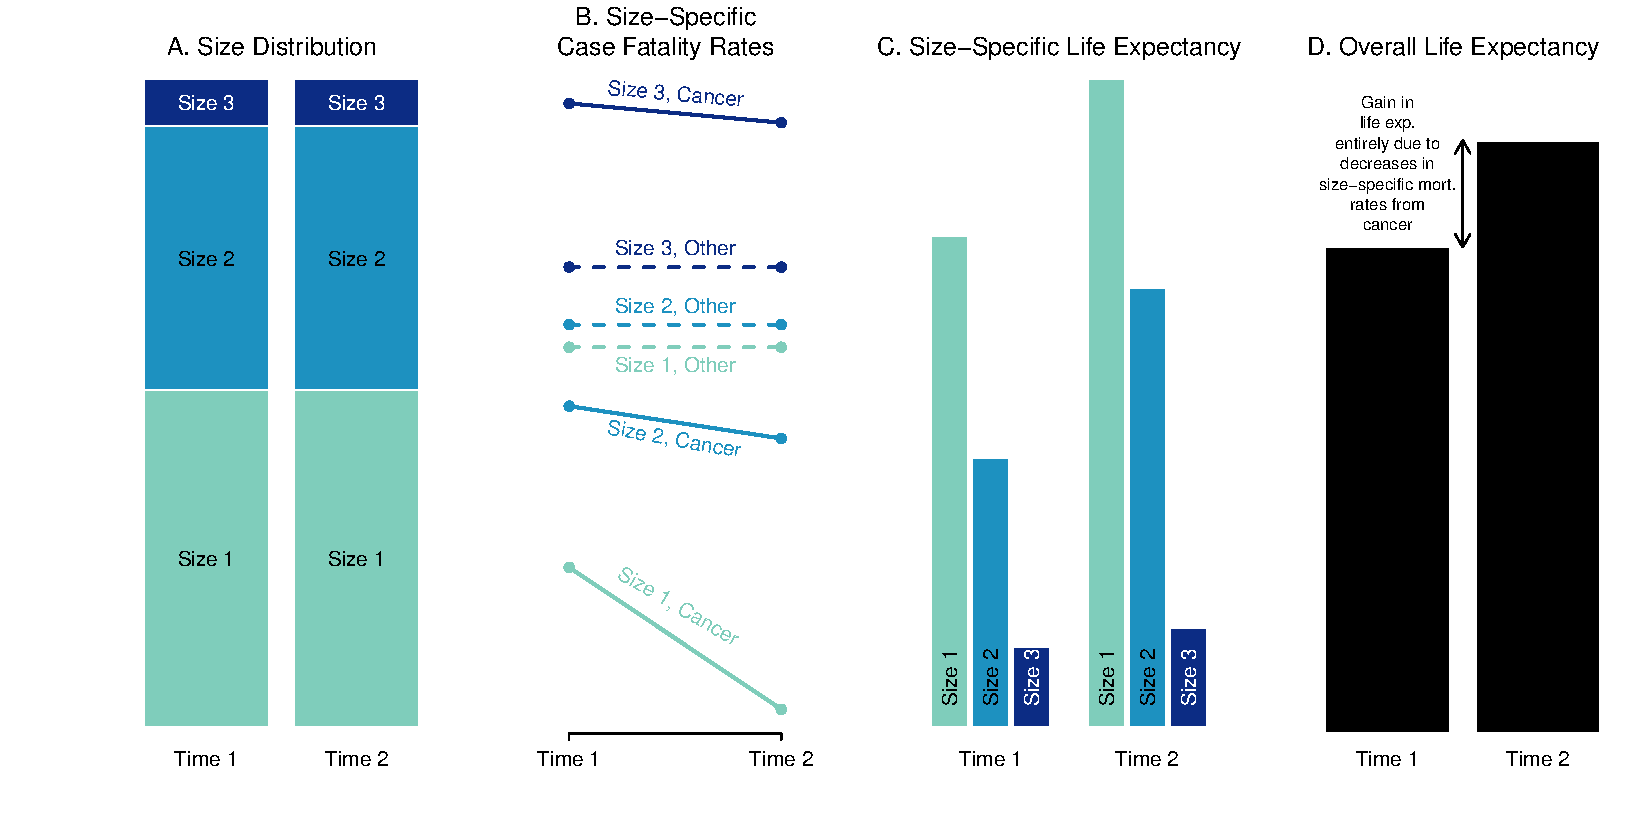
\includegraphics[width=\linewidth]{figure1}
\spacingset{1}\caption{Breast Cancer Incidence Rates, Tumor Size
  Distribution, and Case Fatality Rates.  (A) Incidence rates (cases
  per 100,000 person-years) by tumor size, 1975-2002.  (B) Annual
  share of incident breast cancer cases by tumor size, 1975-2002.  (C)
  Incidence-based case fatality rates from breast cancer and from all
  other causes of death, 1975-2002.}
\label{fig:simple_case}
\end{center}
\end{figure}

\subsection{Gains in Life Expectancy}
Life expectancy increased 10.94 years between 1975 and 2002 for a
40-year old newly diagnosed breast cancer patient (Figure 2).  First,
the temporal shift towards smaller sized tumors contributed 2.92 years
to the gain in life expectancy (27\%).  This 2.92 year net
contribution results from offsetting trends in the share of cancers by
tumor size: increasing contributions from the growing share of smaller
sized tumors and decreasing contributions from the shrinking share of
larger sized tumors.  Second, improvements in case fatality rates from
breast cancer contributed 6.79 years to the gain in life expectancy
(62\%).  Specifically, reductions in case fatality rates from breast
cancer contributed 1.12 years for $<$1cm tumors, 2.36 years for 1-2cm
tumors, 1.12 years for 2-3cm tumors, 1.52 years for 3-5cm tumors, and
0.66 years for ≥5cm tumors.  Third, reductions in case fatality rates
from competing causes of death across all tumor sizes contributed the
remaining 1.25 years to the gain in life expectancy (11\%).

\begin{figure}[h]
\begin{center}
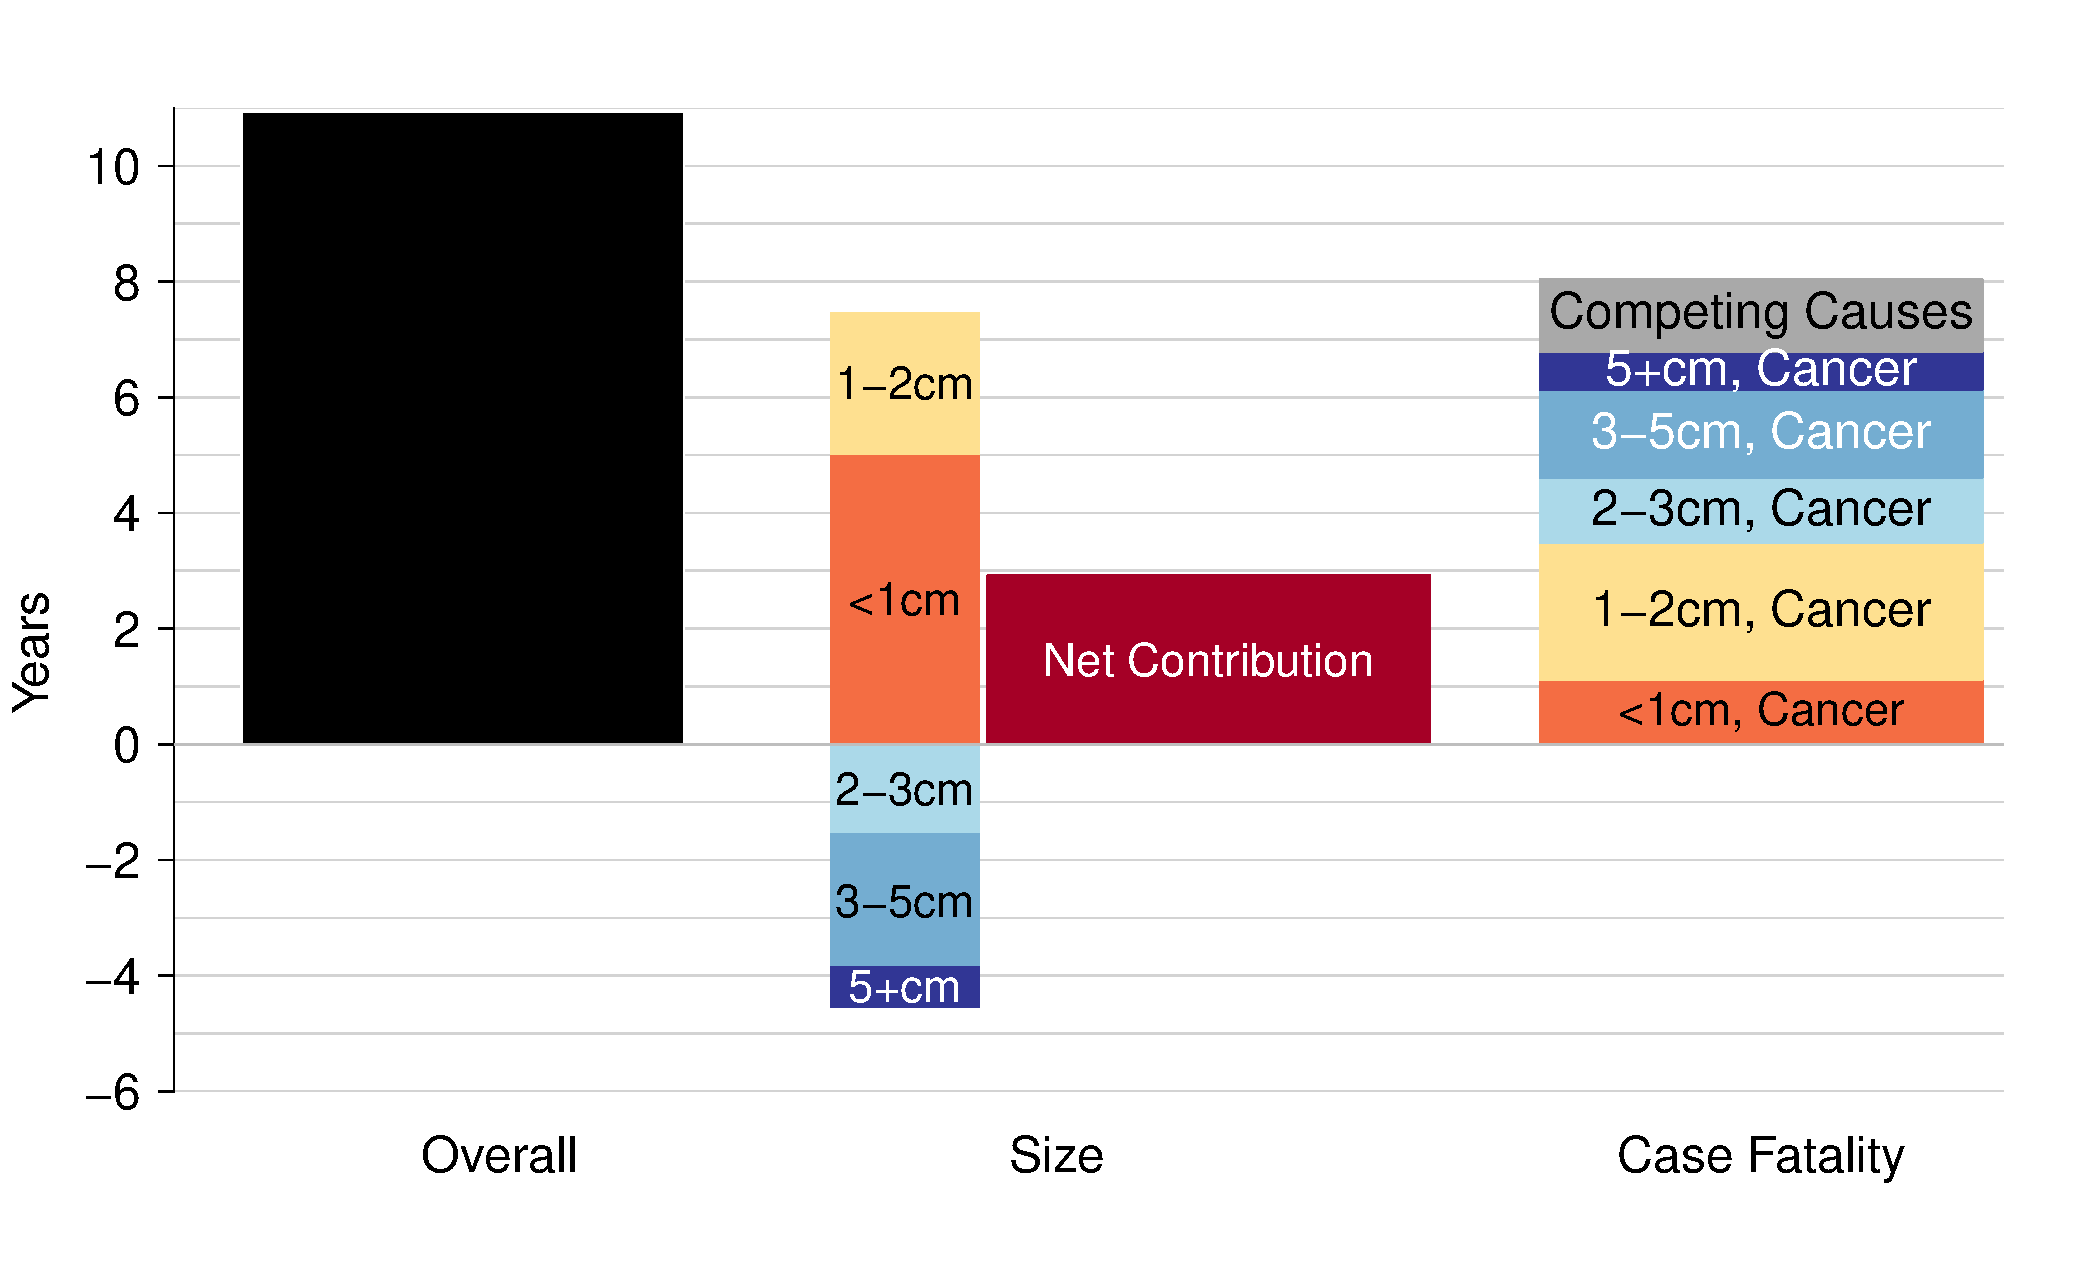
\includegraphics[width=\linewidth]{figure2}
\spacingset{1}\caption{Contribution of Earlier Detection, Advancements
  in Breast Cancer Treatment, and Advancements in Treatment of
  Competing Diseases on Gain in Life Expectancy.  Overall gain in life
  expectancy and the contribution of the temporal shift in tumor size
  (by tumor size and net contribution) and reductions in case fatality
  rates from breast cancer and competing causes of death.}
\label{fig:simple_case}
\end{center}
\end{figure}

\spacingset{2}
\subsection{Contribution by Age Group to Earlier Detection}
The contribution of the temporal shift towards smaller sized tumors
(2.92 years) represents the net of 5.02 years from $<$1cm tumors and
2.43 years from 1-2cm tumors (growing shares) and -4.79 years from
2-3cm, 3-5cm, and ≥5cm tumors (shrinking shares, Table 1).  Of the
overall contribution of the growing share of $<$1 cm tumors, 50-59 years
olds contributed the most followed by 60-69 and 70-79 years
olds. Similarly, of the overall contribution of the growing share of
1-2 cm tumors, 70-79 years olds contributed the most followed by 60-69
and 50-59 years olds. Combining the effect of growing shares of
smaller sized tumors and shrinking shares of larger sized tumors,
earlier detection in 70-79 year olds contributed the most among all
age groups to the net contribution of earlier detection.

\spacingset{1}
\begin{center}
  \begin{table}[h]
\begin{tabular}{@{}l rrrr rrrr@{}}
& \multicolumn{8}{c}{Age Group (Years)}\\ 
 Tumor Size &40-49&50-59&60-69&70-79&80-89&90-99&$\geq$100&Total\\
  \midrule
$<$1cm&0.71&1.35&1.29&1.14&0.49&0.04&0.00&5.02\\
1-2cm&0.29&0.47&0.60&0.62&0.38&0.08&0.00&2.43\\
2-3cm, 3-5 cm, ≥5cm&-0.44&-1.37&-1.48&-1.04&-0.23&0.01&0.00&-4.54\\
  \bottomrule
 Total&0.56&0.45&0.41&0.72&0.65&0.12&0.01&2.92\\
\end{tabular}
\caption{Contribution of Earlier Detection by Age Group.  Note: cm=centimeters.}\end{table}
\end{center}

\spacingset{2}\subsection{Varying Level of Overdiagnosis}  
Our primary analysis assumed an overdiagnosis level of 10\% among
$<$1cm, 1-2cm, and 2-3cm tumors.  In secondary analysis, we varied the
overdiagnosis level among these tumors sizes between 0\% and 52\%
(Figure 3).  As the overdiagnosis level increased, the proportionate
contribution from reductions in case fatality rates from breast cancer
increased while the proportionate contribution from earlier detection
decreased.  For example, at a 20\% overdiagnosis level, the
contributions to the 10.31-year gain in life expectancy were 66\% from
reductions in case fatality rates from breast cancer, 23\% from the
temporal shift to smaller sized tumors, and 12\% from reductions in
case fatality rates from competing causes of death.  We also
independently varied the overdiagnosis level for $<$1cm tumors and 1-3cm
tumors and reached similar conclusions (Supplementary Materials
Section H).
\begin{figure}[h]
\begin{center}
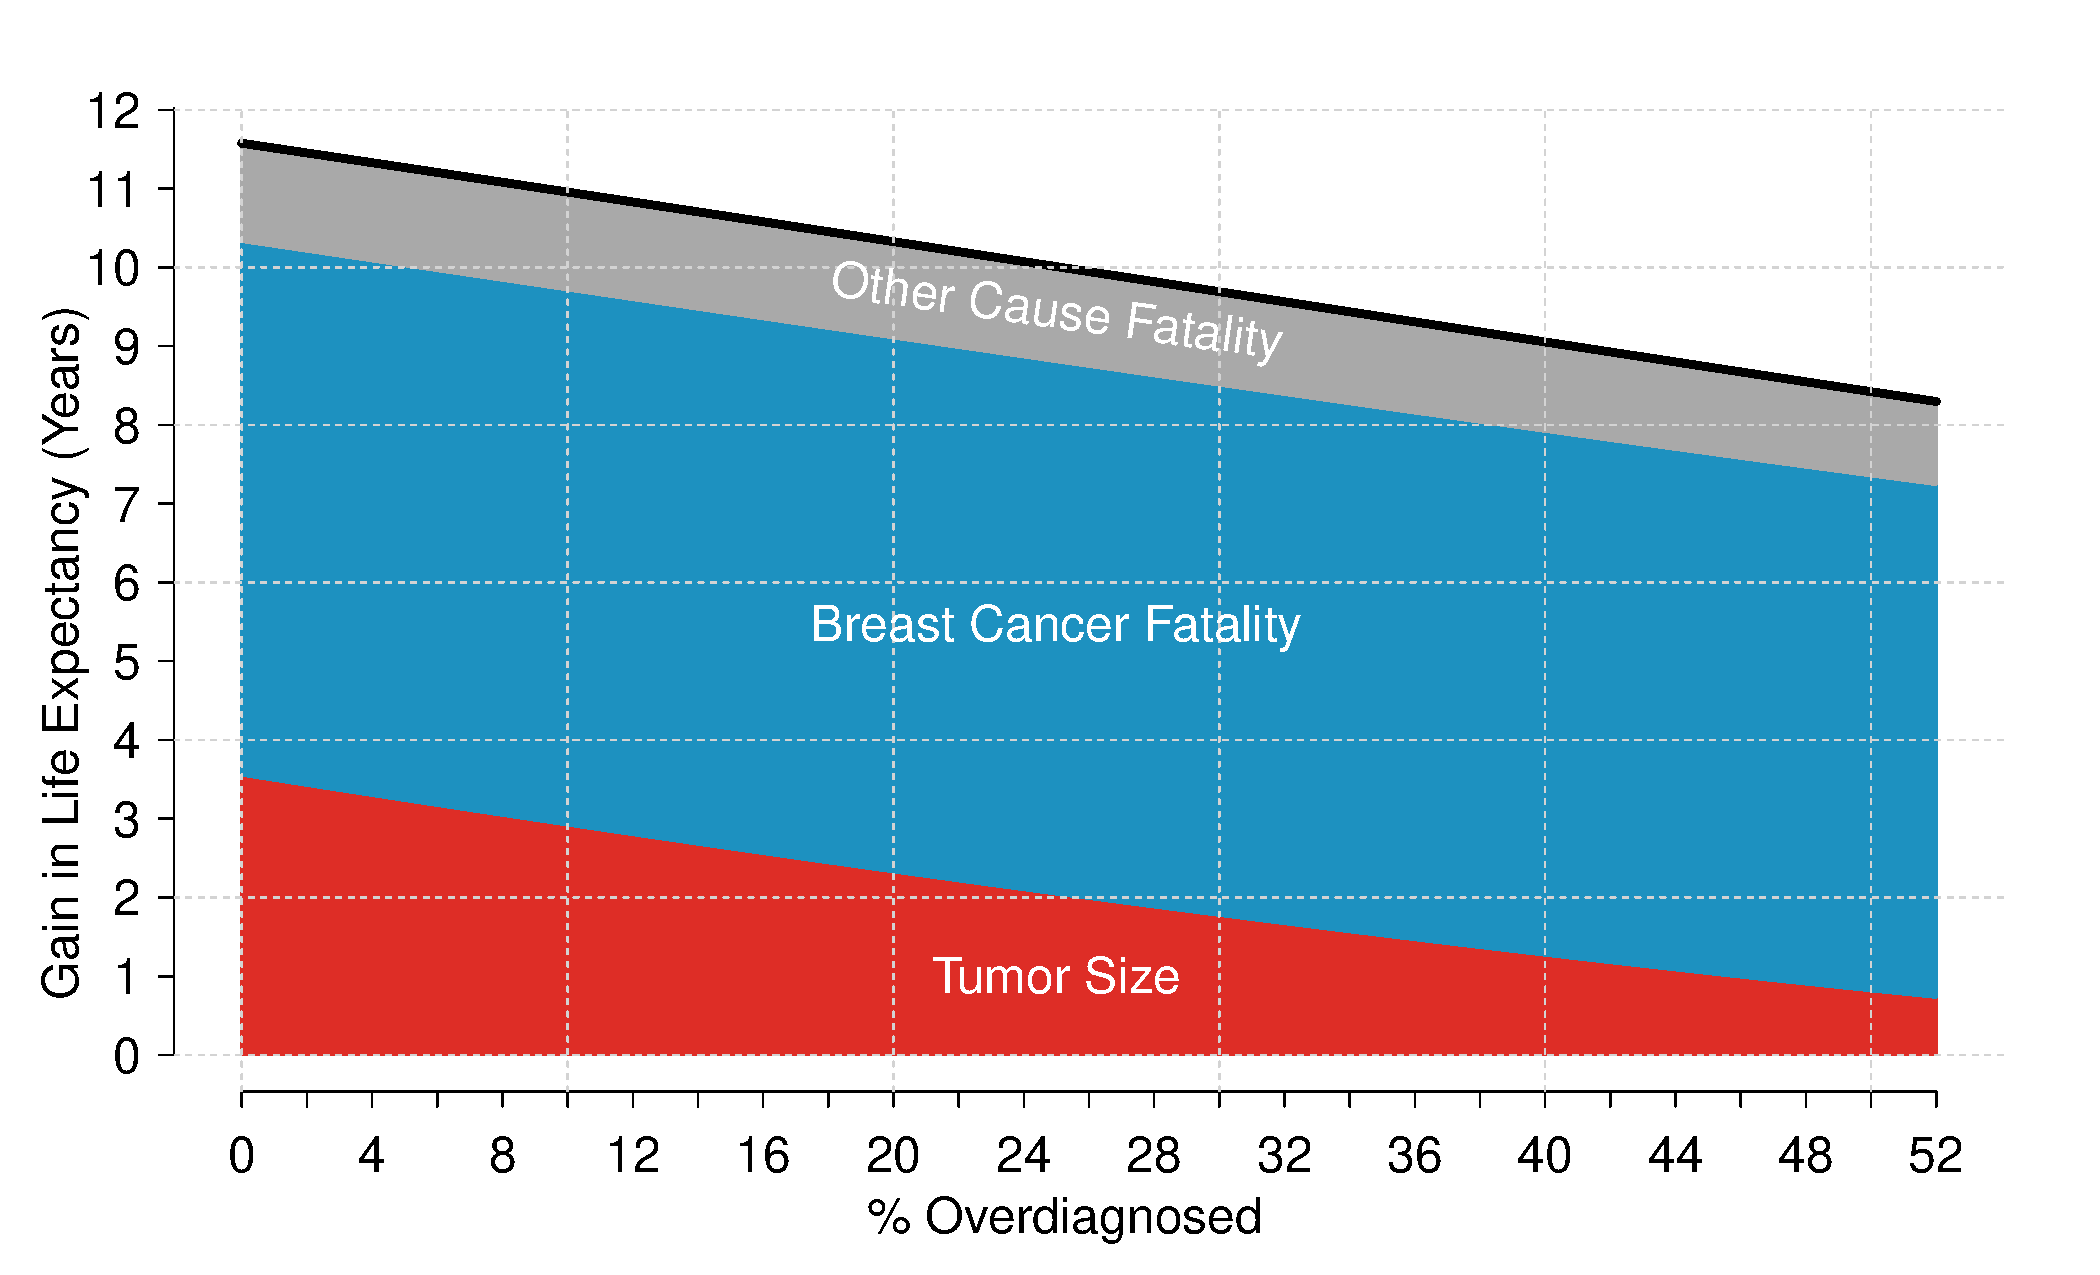
\includegraphics[scale=0.475]{figure3}
\spacingset{1}\caption{Contributions to Gain in Life Expectancy,
  Varying Level of Overdiagnosis.  Overall gain in life expectancy
  and its constituent components (temporal shift in tumor size,
  reductions in case fatality rates from breast cancer, and reductions
  in case fatality rates from competing causes of death) varying the
  level of overdiagnosis for tumors ≤3cm from 0\% to 52\%.}
\label{fig:simple_case}
\end{center}
\end{figure}

\section{Discussion}
Our analysis quantifies the contribution of earlier detection,
advancements in breast cancer treatment, and advancements in the
treatment of other diseases on the gain in life expectancy of US
breast cancer patients.  We show that the majority, 63\%, of the gain
in life expectancy between 1975 and 2002 resulted from advancements in
the breast cancer treatment, which reduced case fatality rates from
breast cancer.  Next, 27\% of the gain resulted from earlier
detection, which increased the share of smaller sized tumors over
time.  Finally, the remaining 12\% of the gain resulted from
advancements in the treatment of other diseases, which reduced case
fatality rates from competing causes of death.  The relative
contribution of each of these three constituent components remained
the same across various levels of overdiagnosis.

Our study adds to a growing body of research on the contribution of
earlier detection on improvements in breast cancer outcomes (21). The
seven simulation-based CISNET models estimated screening contributed
to between 28\% and 65\% of the decline in breast cancer mortality
rates between 1975 and 2000, which corresponds to an equivalent
contribution of between 16\% and 50\% on the resulting gain in life
expectancy (1).  During this same time period, our estimate of the
contribution of earlier detection (24\%), fell on the lower end of the
CISNET range.  Additionally, although the incidence rates of 3-5cm and
≥5cm tumors remained relatively stable since 1990, this constancy does
not necessarily imply screening failed to detect these largest and
most problematic cancers.  Screening only fails to reduce the
incidence of larger sized tumors if we assume the underlying nature of
these cancers is constant over time (i.e., risk factors do not change
over age, time, and across cohorts).  A recent analysis considered
age, time, and cohort effects for metastatic cancer and concluded that
the incidence rate would have increased over time in the absence of
screening; screening reduced this increase to produce the constant
trend observed (23).

Our results also directly address the longstanding controversy over
the value of mammography screening, especially among 40-49 year olds
(2, 24).  Our estimate of the benefit of screening among 40-49 year
olds, which is based on the actual mortality experience of breast
cancer patients, is higher than most previous estimates (25$-–$27).  We
conclude that earlier detection among 40-49 year olds contributed 0.56
of the 10.94-year gain in life expectancy, or 5.16\%.  This
contribution was greater than the corresponding contributions of 50-59
and 60-69 year olds (4.14\% and 3.70\%, respectively).  Previous
estimates of the benefits of screening among 40-49 year olds came from
simulation-based studies, randomized trials, and cross-national
studies.  Yet, simulation studies are based on inherently untestable
assumptions on the natural history of breast cancer (28).  The
efficacy demonstrated in randomized trials may not translate to the
same level of effectiveness in actual populations because of limited
external validity. And cross-national studies are ecological in nature
and based on comparisons of whether women were offered screening
rather than actually screened.

While the contribution from earlier detection on the gain in life
expectancy was substantial, we found that the contribution from
advancements in breast cancer treatment was even larger.
Treatment-related advancements likely resulted from a combination of
improvements in the delivery of existing treatments (e.g.,
breast-conserving surgery with radiotherapy) and the development of
novel treatments (e.g., tamoxifen for breast cancer chemoprevention),
both of which reduced case fatality rates (29, 30).  The same CISNET
models estimated breast cancer treatment contributed to between 35\%
and 72\% of the decline in breast cancer mortality rates or,
equivalently, between 50\% and 84\% of the resulting gain in life
expectancy.  Our estimate of the contribution of advancements in
breast cancer treatment (62\%) fell on the lower end of the CISNET
range.

Advancements in the prevention and treatment of competing causes of
death, such as CVD (31, 32), also contributed to the gain in life
expectancy among breast cancer patients.  After breast cancer itself,
other cancers and CVD were the second and third leading causes of
death among breast cancer patients (33).  For early stage breast
cancers, which are also generally smaller sized tumors, the
probability of death from other causes is considerably higher than the
corresponding probability from breast cancer.  Thus, improvements in
the treatment of other diseases for breast cancer patients are
particularly important for the gain in life expectancy because the
share of smaller sized tumors grew over time.

Our study has some potential limitations.  First, our results may be
subject to bias from misclassification of the underlying cause of
death on death certificates. This bias is unlikely to affect our
results because the accuracy of breast cancer as the cause of death
between medical records and death certificates exceeds 92\% and is
among the highest across all cancer types (34, 35).  Second, our
results may not be generalizable nationally to the extent that the
SEER registries fail to capture national patterns in mammography
screening and breast cancer mortality.  The SEER 9 registries include
both areas of comparatively high and low prevalence of mammography
screening (36).  Additionally, breast cancer mortality patterns in the
SEER registries are highly representative of national breast cancer
mortality patterns (37).  Third, we required that breast cancer death
must have occurred within 10 years of diagnosis when calculating case
fatality rates to partially mitigate the effect of length bias.  We
vary the time interval between 8 years and 12 years and reach
identical substantive conclusions (Supplementary Materials, Section
I).  Finally, we cannot quantify the contribution of individual types
of cancer treatment because patients typically received multiple
modalities for virtually the entire time period of our study (38).

In conclusion, we quantify the benefit of earlier detection and
advancements in breast cancer treatment for US breast cancer patients
between 1975 and 2002.  Earlier detection contributed to more than
one-quarter of the observed gain in life expectancy; advancements in
breast cancer treatment contributed substantially more.  The value of
screening is based on the balance of potential benefits of earlier
detection and potential harms from overdiagnosis and overtreatment.
Our study provides greater clarity to the longstanding debate on the
value of mammography screening by quantifying the realized benefit of
earlier detection against which its potential harms can be measured.

\newpage
\section*{References}
\spacingset{1}
1. 	D. A. Berry et al., Effect of Screening and Adjuvant Therapy
on Mortality from Breast Cancer. N. Engl. J. Med. 353, 1784–1792
(2005).\\\\
2. 	D. B. Kopans, The 2009 U.S. Preventive Services Task Force Guidelines Ignore Important Scientific Evidence and Should Be Revised or Withdrawn. Radiology. 256, 15–20 (2010).\\\\
3. 	D. B. Petitti et al., Breast Cancer Screening: From Science to Recommendation. Radiology. 256, 8–14 (2010).\\\\
4. 	P. C. M. D. Gotzsche, I. Heath, F. Visco, Mammography Screening: Truth, Lies and Controversy (Radcliffe Medical PR, London ; New York, 1 edition., 2012).\\\\
5. 	D. Berry, Breast cancer screening: Controversy of impact. Breast. 22, S73–S76 (2013).\\\\
6. 	A. B. Miller et al., Twenty five year follow-up for breast cancer incidence and mortality of the Canadian National Breast Screening Study: randomised screening trial. BMJ. 348, g366 (2014).\\\\
7. 	Harding C et al., Breast cancer screening, incidence, and mortality across us counties. JAMA Intern. Med. (2015), doi:10.1001/jamainternmed.2015.3043.\\\\
8. 	H. D. Nelson et al., Screening for Breast Cancer: An Update for the U.S. Preventive Services Task Force. Ann. Intern. Med. 151, 727–737 (2009).\\\\
9. 	E. Sun et al., The Contributions of Improved Therapy and Earlier Detection to Cancer Survival Gains, 1988-2000. Forum Health Econ. Policy. 13 (2010). \\\\
10. 	M. A. Helvie, Digital Mammography Imaging: Breast Tomosynthesis and Advanced Applications. Radiol. Clin. North Am. 48, 917–929 (2010).\\\\
11. 	H. Beltrán-Sánchez, S. H. Preston, V. Canudas-Romo, An integrated approach to cause-of-death analysis: cause-deleted life tables and decompositions of life expectancy. Demogr. Res. 19, 1323–1350 (2008).\\\\
12. 	Samir Soneji, Hiram Beltrán-Sánchez, Harold Sox, Assessing Progress in Reducing the Burden of Cancer Mortality, 1985-2005. J. Clin. Oncol. 32, 444–448 (2014).\\\\
13. 	K. C. Chu, B. A. Miller, E. J. Feuer, B. F. Hankey, A method for partitioning cancer mortality trends by factors associated with diagnosis: an application to female breast cancer. J. Clin. Epidemiol. 47, 1451–1461 (1994).\\\\
14. 	K. C. Chu, R. E. Tarone, H. P. Freeman, Trends in prostate cancer mortality among black men and white men in the United States. Cancer. 97, 1507–1516 (2003).\\\\
15. 	S. Zackrisson, I. Andersson, L. Janzon, J. Manjer, J. P. Garne, Rate of over-diagnosis of breast cancer 15 years after end of Malmö mammographic screening trial: follow-up study. BMJ. 332, 689–692 (2006).\\\\
16. 	E. M. Kitagawa, Components of a Difference Between Two Rates*. J. Am. Stat. Assoc. 50, 1168–1194 (1955).\\\\
17. 	S. H. Preston, P. Heuveline, M. Guillot, Demography: Measuring and Modeling Population Processes (Blackwell Publishers Ltd, 2001).\\\\
18. 	M.-F. Yen et al., Quantifying the potential problem of overdiagnosis of ductal carcinoma in situ in breast cancer screening. Eur. J. Cancer Oxf. Engl. 1990. 39, 1746–1754 (2003).\\\\
19. 	K. J. Jørgensen, P. C. Gøtzsche, Overdiagnosis in publicly organised mammography screening programmes: systematic review of incidence trends. BMJ. 339, b2587 (2009).\\\\
20. 	H. G. Welch, W. C. Black, Overdiagnosis in Cancer. J. Natl. Cancer Inst. 102, 605–613 (2010).\\\\
21. 	M. Kalager, M. Zelen, F. Langmark, H.-O. Adami, Effect of screening mammography on breast-cancer mortality in Norway. N. Engl. J. Med. 363, 1203–1210 (2010).\\\\
22. 	R. Etzioni, J. Xia, R. Hubbard, N. S. Weiss, R. Gulati, A Reality Check for Overdiagnosis Estimates Associated With Breast Cancer Screening. J. Natl. Cancer Inst. 106, dju315 (2014).\\\\
23. 	R. E. Gangnon et al., The contribution of mammography screening to breast cancer incidence trends in the United States: an updated age-period-cohort model. Cancer Epidemiol. Biomark. Prev. 24, 905–912 (2015). \\\\
24. 	P. C. Gøtzsche, O. Olsen, Is screening for breast cancer with mammography justifiable? Lancet. 355, 129–134 (2000). \\\\
25. 	S. M. Moss et al., Effect of mammographic screening from age 40 years on breast cancer mortality in the UK Age trial at 17 years’ follow-up: a randomised controlled trial. Lancet Oncol. (2015).\\\\
26. 	B. Lauby-Secretan et al., Breast-cancer screening--viewpoint of the IARC Working Group. N. Engl. J. Med. 372, 2353–2358 (2015). \\\\
27. 	US Preventive Services Task Force, “Draft Recommendation Statement: Breast Cancer: Screening” (2015).\\\\
28. 	N. K. Stout, A. B. Knudsen, C. Y. (Joey) Kong, P. M. McMahon, G. S. Gazelle, Calibration Methods Used in Cancer Simulation Models and Suggested Reporting Guidelines. PharmacoEconomics. 27, 533–545 (2009). \\\\
29. 	Consensus statement: treatment of early-stage breast cancer. National Institutes of Health Consensus Development Panel. J. Natl. Cancer Inst. Monogr., 1–5 (1992). \\\\
30. 	B. Fisher et al., Tamoxifen for Prevention of Breast Cancer: Report of the National Surgical Adjuvant Breast and Bowel Project P-1 Study. J. Natl. Cancer Inst. 90, 1371–1388 (1998). \\\\
31. 	Hunink MM, Goldman L, Tosteson AA, et al, The recent decline in mortality from coronary heart disease, 1980-1990: The effect of secular trends in risk factors and treatment. JAMA. 277, 535–542 (1997). \\\\
32. 	M. L. Weisfeldt, S. J. Zieman, Advances In The Prevention And Treatment Of Cardiovascular Disease. Health Aff. (Millwood). 26, 25–37 (2007). \\\\
33. 	C. Schairer, P. J. Mink, L. Carroll, S. S. Devesa, Probabilities of Death From Breast Cancer and Other Causes Among Female Breast Cancer Patients. J. Natl. Cancer Inst. 96, 1311–1321 (2004). \\\\
34. 	C. Percy, E. Stanek, L. Gloeckler, Accuracy of cancer death certificates and its effect on cancer mortality statistics. Am. J. Public Health. 71, 242–250 (1981). \\\\
35. 	R. R. German et al., The accuracy of cancer mortality statistics based on death certificates in the United States. Cancer Epidemiol. 35, 126–131 (2011). \\\\
36. 	K. L. Schneider, K. L. Lapane, M. A. Clark, W. Rakowski, Using Small-Area Estimation to Describe County-Level Disparities in Mammography. Prev. Chronic. Dis. 6 (2009).\\\\
37. 	R. M. Merrill, K. A. Dearden, How representative are the surveillance, epidemiology, and end results (SEER) Program cancer data of the United States? Cancer Causes Control. 15, 1027–1034 (2004). \\\\
38. 	G. Bonadonna et al., Combination Chemotherapy as an Adjuvant Treatment in Operable Breast Cancer. N. Engl. J. Med. 294, 405–410 (1976).










\setcounter{table}{0} % reset counter for equation numbers
\setcounter{figure}{0} % reset counter for equation numbers
%\setcounter{page}{1} 
\renewcommand{\figurename}{Supplemental Figure}
\renewcommand{\tablename}{Supplemental Table}
%\clearpage
%\pagenumbering{gobble}
\appendix
\newpage
\spacingset{2}
\section*{Supplementary Materials}
\section{Computation of Incidence-Based Case Fatality Rates}
An incidence-based case fatality rate for a specific cohort of newly
diagnosed breast cancer patients equals the ratio of [1] the number of
deaths occurring for this cohort up to 10 years beyond their diagnosis
and [2] the total number of person-years lived by this cohort up to 10
years beyond their diagnosis.  For example, 556 women aged 65-69 years
were diagnosed with $<$1cm breast cancer in 2001.  Between 2001 and
2011, 22 of these women died of breast cancer and another 107 died of
a competing cause of death.  This entire cohort lived a total of
5099.5 person-years over the 10-year period.  Thus, the
incidence-based case fatality rate from breast cancer equaled
22/5099.5 and the incidence-based case fatality rate from competing
causes of death equaled 107/5099.5.  Also, the proportion of women
diagnosed with $<$1cm breast cancer in 2001 equaled 4,602 out of 19,029
newly diagnosed breast cancers (24.2\%).

\section{Adjustment for Overdiagnosis}
Suppose 10\% of the 556 women aged 65-69 years old diagnosed with $<$1cm
breast cancer in 2001 were overdiagnosed, the observed case fatality
rate from breast cancer (22/5099.5) would become 22/[5099.5 -
0.10*5099.5].  Formally, let $\mathcal{A}$ be a set of starting ages
for age intervals analyzed (e.g., 40, 45, \dots, $\omega=100$ years), $\mathcal{T}$ be a set of
years (e.g., 1975, \dots 2002), and $\mathcal{S}$ be a set of tumor
sizes at diagnosis (e.g., $<$1cm, 1-2cm, 2-3cm, 3-5cm, and $\geq5$cm).
Let $\alpha_s$ represent the assummed level of overdiagnosis for tumor
size $s\in\mathcal{S}$.  Let $m_{a,t,s}$ represent the observed case
fatality rate for age group $a \in \mathcal{A}$, year $t \in
\mathcal{T}$, and tumor size $s \in \mathcal{S}$.  Then, the case
fatality rate adjusted for overdiagnosis, $m^*_{a,t,s}$, equals,
$\frac{1}{1-\alpha_s} \times m_{a,t,s}$.

In 2001, the number of women diagnosed with breast cancer equaled:
4602 with $<$1cm tumors, 7208 with 1-2cm tumors, 3684 with 2-3cm
tumors, and 1300 with $\geq5$cm tumors.  These counts translate to the
following distribution: 24\%, 38\% 19\%, 12\%, and 7\%, respectively.
Suppose 10\% of $<$1cm breast cancers were overdiagnosed (460 of 4602
women).  We subtract these 460 women from the count of breast cancers
in 2001 and recalculate the distribution: 22\% for $<$1cm, 39\% for
1-2cm, 20\% for 2-3cm, 12\% for 3-5cm, and 7\% for $\geq5$cm.  
Let $\alpha_s$ represent the assummed level of overdiagnosis for tumor
size $s\in\mathcal{S}$.  Let $n_{t,s}$ represent the observed count
of breast cancer cases in year $t$ and for tumor size $s$.  The
observed distribution of incident breast cancer cases, $\pi_{t,s}$, equals
$\frac{n_{t,s}}{\sum_{s\in\mathcal{S}}n_{t,s}}$.  The distribution of
incident breast cancer cases adjusted for overdiagnosis equals: 
\begin{eqnarray}
\pi^*_{t,s}=\frac{(1-\alpha_s) \times n_{t,s}}{\sum_{s\in\mathcal{S}}
  (1-\alpha_s) \times n_{t,s}} \notag.
\end{eqnarray} 

\section{Computation of Tumor Size-Specific Life Expectancy}
The life expectancy of a breast cancer patient newly diagnosed at age
$a^*\in\mathcal{A}$, at time $t$, and with tumor size $s$ equals:
\begin{eqnarray}
 e_s(a^*,t)=\int_{a^*}^{\omega} e^{\left( -\int_{a*}^{a}\mu_s(y,t)\,dy \right)}da =\int_{a^*}^{\omega} e^{\left(-\sum_{a=a*}^{a}n\,m^*_{a,t,s}\right)}\,da ,
\end{eqnarray} 
where $\mu_s(a,t)$ and $m^*_{a,t,s}$ represent the hazard of mortality
and case fatality rate adjusted for overdiagnosis, respectively; $n$
is the width of the age interval; and $\omega$ is the starting age of
the final and open-ended age interval.

\section{Schematic Representation of the Methodology}
For simplicity, consider three mutually exclusive and exhaustive
categories of tumor size: 1, 2, and 3 (e.g., $<$1cm, 1-2cm, and
$\geq$2cm).  Suppose the distribution of tumor size at cancer
diagnosis remained constant between times 1 and 2 (Supplemental
Figure~\ref{fig:simple_case}, Panel A), tumor size-specific case
fatality rates from breast cancer decreased between times 1 and 2
(Supplemental Figure~\ref{fig:simple_case}, Panel B), and tumor
size-specific case fatality rates from competing causes of death
remained constant between times 1 and 2 (Supplemental
Figure~\ref{fig:simple_case}, Panel B).  Tumor size-specific life
expectancy increased between times 1 and 2 because tumor size-specific
case fatality rates from breast cancer decreased over the time period
(Supplemental Figure~\ref{fig:simple_case}, Panel C).  Overall life
expectancy at each time equals the weighted average of tumor
size-specific life expectancy, where the weights equal the
distribution of tumor sizes at cancer diagnosis at times 1 and 2,
respectively.  Overall life expectancy grew between times 1 and 2, and
this gain was entirely due to decreases in tumor size-specific case
fatality rates from breast cancer (Supplemental
Figure~\ref{fig:simple_case}, Panel D).  In actuality, all three
aforementioned factors change over time and contribute to the gain in
life expectancy.  We quantify the individual contribution of each of
these three constituent components.  We also utilize the same
demographic method to further disaggregate these three contributions
by age group in Section~\ref{sec:age}.
\begin{figure}[h]
\begin{center}
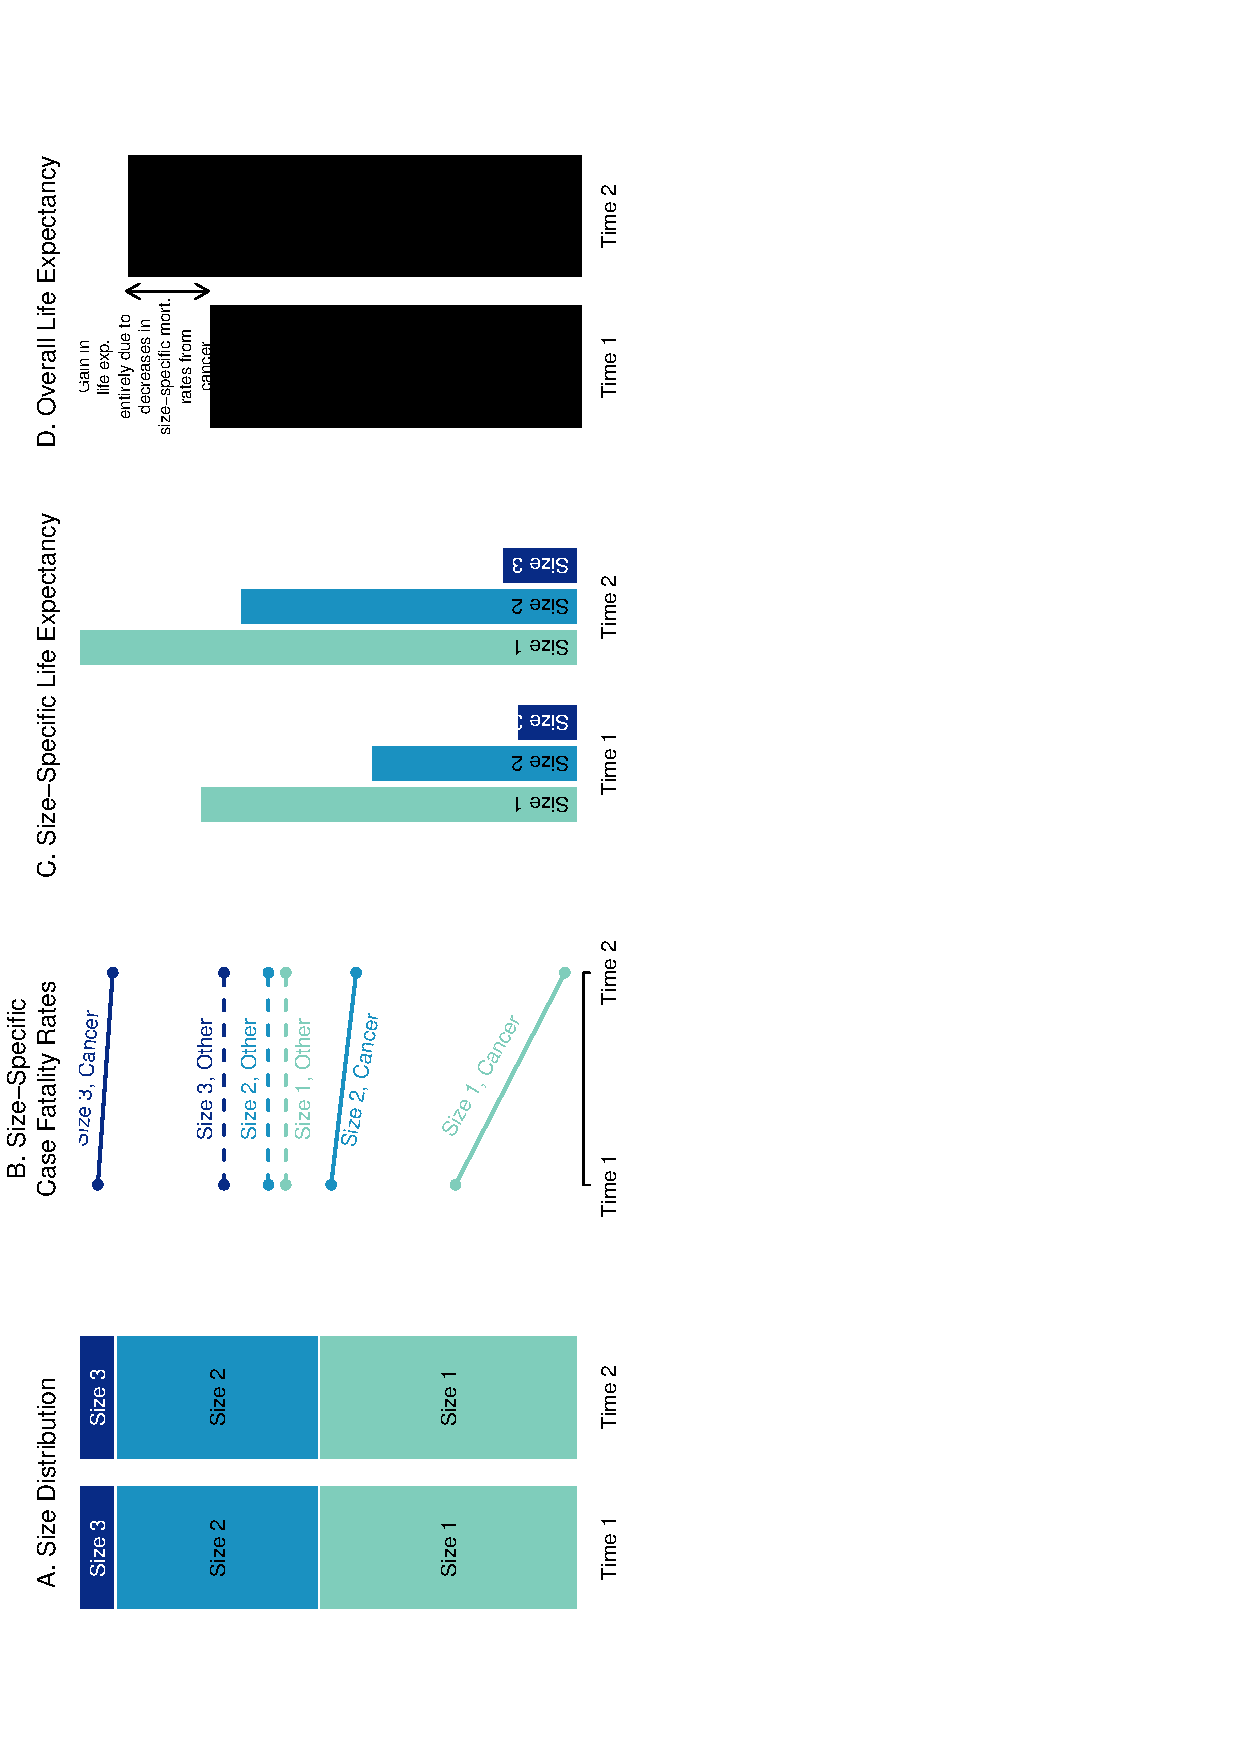
\includegraphics[trim=0 220 0 0,clip,width=\linewidth]{appendix_figure1}
\spacingset{1}\caption{The gain in life expectancy depends
  on three factors: (A) changes in the tumor size distribution at
  cancer diagnosis, (B) changes in tumor size-specific case fatality rates from
  breast cancer, and (C) changes in tumor size-specific case fatality rates from
  competing causes of death.}
\label{fig:simple_case}
\end{center}
\end{figure}

\section{Decomposition by Tumor Size and Case Fatality Rates from
  Breast Cancer and Other Causes of Death}
Let $\pi_s(t)$ equal the proportion of breast cancer patients
diagnosed with tumor size $s$ in year $t$.  Let $e_s(a,t)$ equal the
tumor size-specific life expectancy at age $a$. The overall life
expectancy at age $a$ and time $t$, $e(a,t)$, equals:
\begin{eqnarray}
  e(a,t)=\sum_{s\in\mathcal{S}}\,\pi_s(t)\,e_s(a,t), \notag
\end{eqnarray}
where $\sum_{s\in\mathcal{S}}\,\pi_s=1$. 

The change in life expectancy at age $a$ between times $t_1$ and $t_2$
can be decomposed using the methodology of \cite{Kitagawa55}:
\begin{align}
  e(a,t_2)-e(a,t_1)&=\sum_{s\in\mathcal{S}}\left[\,\pi_s(t_2)\,e_s(a,t_2)- \pi_s(t_1)\,e_s(a,t_1)\right]  \notag\\
  \hspace{-0.7in} &=\sum_{s\in\mathcal{S}}\left[\pi_s(t_2)-\pi_s(t_1)
  \right]\left[\frac{e_s(a,t_1)+e_s(a,t_2)}{2}\right]+ \notag\\
  &\phantom{=}\sum_{s\in\mathcal{S}}\left[e_s(a,t_2)-e_s(a,t_1)
  \right]\left[\frac{\pi_s(t_1)+\pi_s(t_2)}{2}\right].
 \label{eqn:decomp.basic}
\end{align}
 
Equation~\ref{eqn:decomp.basic} quantifies how much of the change in life
expectancy at age $a$ between times $t_1$ and $t_2$ is due to: [a]
shifts in the share of cancer tumor size (first term) and [b] changes
in tumor-size-specific life expectancy (second term).

We can further decompose the second term of
equation~\ref{eqn:decomp.basic} by cause of death. In doing so, we can
quantify how much of this change in tumor-size-specific cancer life
expectancy, $e_s(a,t_2)-e_s(a,t_1)$, is due to improvements in case
fatality rates from breast cancer and improvements in case fatality
rates from  competing causes of death.  Let $\mathcal{C}$ be a set of
mutually exclusive and exhaustive causes of death (e.g., breast cancer
and all other causes).  Let $L_{a,s,c}(t)$ represent the person-years
lived in the life table based on the case fatality rate at age $a$,
for tumor size $s$, from cause $c\in\mathcal{C}$, and at time $t$.
Similarly, let $L_{a,s,-c}(t)$ represent the person-years lived in the
life table based on the case fatality rate at age $a$, for tumor size
$s$, and from causes other than $c$ ($-c$), and at time $t$.  Let $a^*$ be
the first starting age of $\mathcal{A}$.  Then, following the approach
developed by \cite{BelPreCan08},
\begin{eqnarray}
e_s(a^*,t_2)-e_s(a^*,t_1)= \sum_{c\in\mathcal{C}}\sum_{a=a^*}^\omega \left[L_{a,s,c}(t_2)-L_{a,s,c}(t_1) \right] \left[\frac{L_{a,s,-c}(t_2)+L_{a,s,-c}(t_1) }{2n} \right],
\label{eqn:causedecomp}
\end{eqnarray}
where $n$ is the width of the age interval and $\omega$ is the
starting age of the final and open-ended age interval.

We perform the decomposition starting at age 40; the final
decomposition equation equals:
\begin{align*}
  e(40,t_2)-e(40,t_1)&=\sum_{s\in\mathcal{S}}\left[\,\pi_s(t_2)\,e_s(40,t_2)- \pi_s(t_1)\,e_s(40,t_1)\right] \notag \\
                     &=\sum_{s\in\mathcal{S}}\left[\pi_s(t_2)-\pi_s(t_1) \right]\left[\frac{e_s(40,t_1)+e_s(40,t_2)}{2}\right]+\sum_{s\in\mathcal{S}}\left[\mathtt{Diff_e} \right]\left[\frac{\pi_s(t_1)+\pi_s(t_2)}{2}\right],
\end{align*}
where $\mathtt{Diff_e}$ is given by \eqref{eqn:causedecomp} evaluated at $a^*=40$.\\


\section{Decomposition by Tumor Size, Case Fatality Rates from
  Breast Cancer and Other Causes of Death, and Age Group}
\label{sec:age}
As previously defined $\pi_{s}(t)$ equals the proportion of cancer patients with tumor size
$s$ in year $t$. This proportion can also be computed by age group
such that $\pi_s(t)=\sum_{a\in\mathcal{A}}\pi_{s,a}(t)$ and
$\sum_{s\in\mathcal{S}}\,\pi_s=1$.  Then, the
change in life expectancy at age $a$ between times $t_1$ and $t_2$ can
be estimated as:
\begin{align*}
  e(40,t_2)-e(40,t_1)&=\sum_{s\in\mathcal{S}}\left[\,\pi_s(t_2)\,e_s(40,t_2)- \pi_s(t_1)\,e_s(40,t_1)\right] \\
                     &=\sum_{s\in\mathcal{S}} \left[\sum_{a\in\mathcal{A}}\pi_{s,a}(t_2)\,e_s(40,t_2)- \sum_{a\in\mathcal{A}}\pi_{s,a}(t_1)\,e_s(40,t_1) \right]\\
                     &=\sum_{s\in\mathcal{S}}\left[\pi_{s,40}(t_2)\,e_s(40,t_2)-
                       \pi_{s,40}(t_1)\,e_s(40,t_1)\right] +\\
                     &\hspace{0.18in}\sum_{s\in\mathcal{S}}\left[\pi_{s,45}(t_2)\,e_s(40,t_2)- \pi_{s,45}(t_1)\,e_s(40,t_1)\right] + \\
  &\phantom{=\Sigma}\vdots \\
                     &\hspace{0.18in}\sum_{s\in\mathcal{S}}\left[\pi_{s,\omega}(t_2)\,e_s(40,t_{\omega})- \pi_{s,\omega}(t_1)\,e_s(40,t_1)\right]. \notag 
 \end{align*}


 Each summation in the above equation can be written as follows based
 on equation \eqref{eqn:decomp.basic}:
\begin{multline}
  e(40,t_2)-e(40,t_1)= \\
  \sum_{s\in\mathcal{S}}\left[\pi_{s,40}(t_2)-\pi_{s,40}(t_1) \right]\left[\frac{e_s(40,t_1)+e_s(40,t_2)}{2}\right]+\sum_{s\in\mathcal{S}}\left[e_s(40,t_2)-e_s(40,t_1) \right]\left[\frac{\pi_{s,40}(t_1)+\pi_{s,40}(t_2)}{2}\right] +\\
  \sum_{s\in\mathcal{S}}\left[\pi_{s,45}(t_2)-\pi_{s,45}(t_1) \right]\left[\frac{e_s(40,t_1)+e_s(40,t_2)}{2}\right]+\sum_{s\in\mathcal{S}}\left[e_s(40,t_2)-e_s(40,t_1) \right]\left[\frac{\pi_{s,45}(t_1)+\pi_{s,45}(t_2)}{2}\right] +\\
  \vdots \\
  \sum_{s\in\mathcal{S}}\left[\pi_{s,{\omega}}(t_2)-\pi_{s,{\omega}}(t_1) \right]\left[\frac{e_s(40,t_1)+e_s(40,t_2)}{2}\right]+\sum_{s\in\mathcal{S}}\left[e_s(40,t_2)-e_s(40,t_1) \right]\left[\frac{\pi_{s,{\omega}}(t_1)+\pi_{s,{\omega}}(t_2)}{2}\right] =\\
  \sum_{s\in\mathcal{S}}\left[\mathtt{Diff_{\pi,40}} \right]\mathtt{\bar{e}_s} + \sum_{s\in\mathcal{S}}\left[\mathtt{Diff_{\pi,45}} \right]\mathtt{\bar{e}_s} + 
  \dots +
 \sum_{s\in\mathcal{S}}\left[\mathtt{Diff_{\pi,{\omega}}} \right]\mathtt{\bar{e}_s} +\sum_{s\in\mathcal{S}}\left[e_s(40,t_2)-e_s(40,t_1)\right]\left[\frac{\pi_s(t_1)+\pi_s(t_2)}{2}\right]
\label{agedec}
\end{multline}
where $\mathtt{Diff_{\pi,a}}=\pi_{s,a}(t_2)-\pi_{s,a}(t_1)$ and $\mathtt{\bar{e}_i}=\frac{e_s(40,t_1)+e_s(40,t_2)}{2}$.

The terms of equation\eqref{agedec} that include
$\mathtt{Diff_{\pi,40}}\dots \mathtt{Diff_{\pi,\omega}}$ correspond to
the contribution of changes in the share of tumor size by age group to
the change in cancer life expectancy between times $t_1$ and $t_2$.
We can additionally estimate the contribution of changes in case
fatality rates from breast cancer and competing causes of death to
changes in tumor-size-specific life expectancy by age. The last term
of \eqref{agedec} can be written as follows, based on equation
\eqref{eqn:causedecomp}:
\begin{align}
  e_s(40,t_2)-e_s(40,t_1)&=\sum_{c\in\mathcal{C}} \sum_{a=40}^\omega\left[L_{a,s,c}(t_2)-L_{a,s,c}(t_1) \right] \left[\frac{L_{a,s,-c}(t_2)+L_{a,s,-c}(t_1) }{2n} \right].  
\end{align}

\section{Assuming Constant Mortality Within Age Intervals}
Let $M_{a,a+n}$ represent the mortality rate between ages $a$ and
$a+n$ and let $\mu(a)$ represent the hazard of mortality at age
$a$. Then, the number (or proportion) of survivors at age $a+n$ in the
life table, $l_{a+n}$, equals (\cite{PreHeuGui00}):
\begin{equation}
l_{a+n}=l_{a}\,e^{-\int_a^{a+n}\mu(x)\,dx}=l_{a}\,e^{-n\,M_{a,a+n}}.\notag
\end{equation}
Then, the number of person-years lived between ages $a$ and $a+n$ equals:
\begin{equation}
_nL_{a}=l_a\,\int_a^{a+n} e^{-M_{a,a+n}(s-a)} ds=l_a \left(\frac{-1}{M_{a,a+n}}(e^{-n\,M_{a,a+n}}-1) \right).
\label{Lx}
\end{equation}
Suppose the age interval is $n=5$ years wide, then equation \eqref{Lx}
equals:
\begin{equation}
_5L_{a}=l_a \left(\frac{-1}{M_{a,a+5}}(e^{-5\,M_{a,a+5}}-1) \right).\notag
\end{equation}
For the last and open-ended age group (e.g., $\geq$100 years), we can assume there
are no person-years lived beyond a certain time (say no more than 10
years) to compute $_{\infty}L_{100}$ as:
\begin{equation}
_{\infty}L_{100}=l_{100} \left(\frac{-1}{M_{100+}}(e^{-10\,M_{100+}}-1) \right).\notag
\end{equation}

%Consider tumor size $i$.  The change
%in life expectancy at age $x$ between times $t_1$ and $t_2$ can be
%decomposed as (Kitigawa 1955): 
%\begin{equation}
% e_s(x,t_2)-e_s(x,t_1) = \sum_{j=1}^k \int_x^\infty \left[ p_{s,j}(s,t_2)- p_{s,j}(s,t_1)\right] \left[ \frac{p_{s,-j}(s,t_1)+p_{s,-j}(s,t_2)}{2} \right]\,ds, \notag
%\end{equation}
%where $p_{s,j}(s,t)$ is the probability of surviving from birth to age
%$s$ for cancer patients with tumor size $i$ cause $j$ at time $t$, and
%$p_{s,-j}(s,t)$ is the analogue survival probability for competing
%causes of death (other than $j$). 

\newpage
\section{Varying Overdiagnosis Level for $<$1cm and $1-3$cm Tumors}
We individually varied the overdiagnosis level from 0\% to 97\% for
tumors $<$1cm and from 0\% to 52\% for 1-3cm tumors.  We set the upper
bound based on the smallest percentage of patients diagnosed with $<$1cm
tumors who subsequently died of breast cancer within 10 years (3\%).
For example, at overdiagnosis levels of 97\% for $<$1cm tumors and
35\% for 1-3cm tumors, the contribution to the 7.58-year gain in life
expectancy were: 6.40 years from reductions in case fatality rates
from breast cancer (84\%), 0.22 years from the temporal shift to
smaller sized tumors (3\%), and 0.98 years from reductions in case
fatality rates from competing causes of death (13\%).

\begin{figure}[h]
\begin{center}
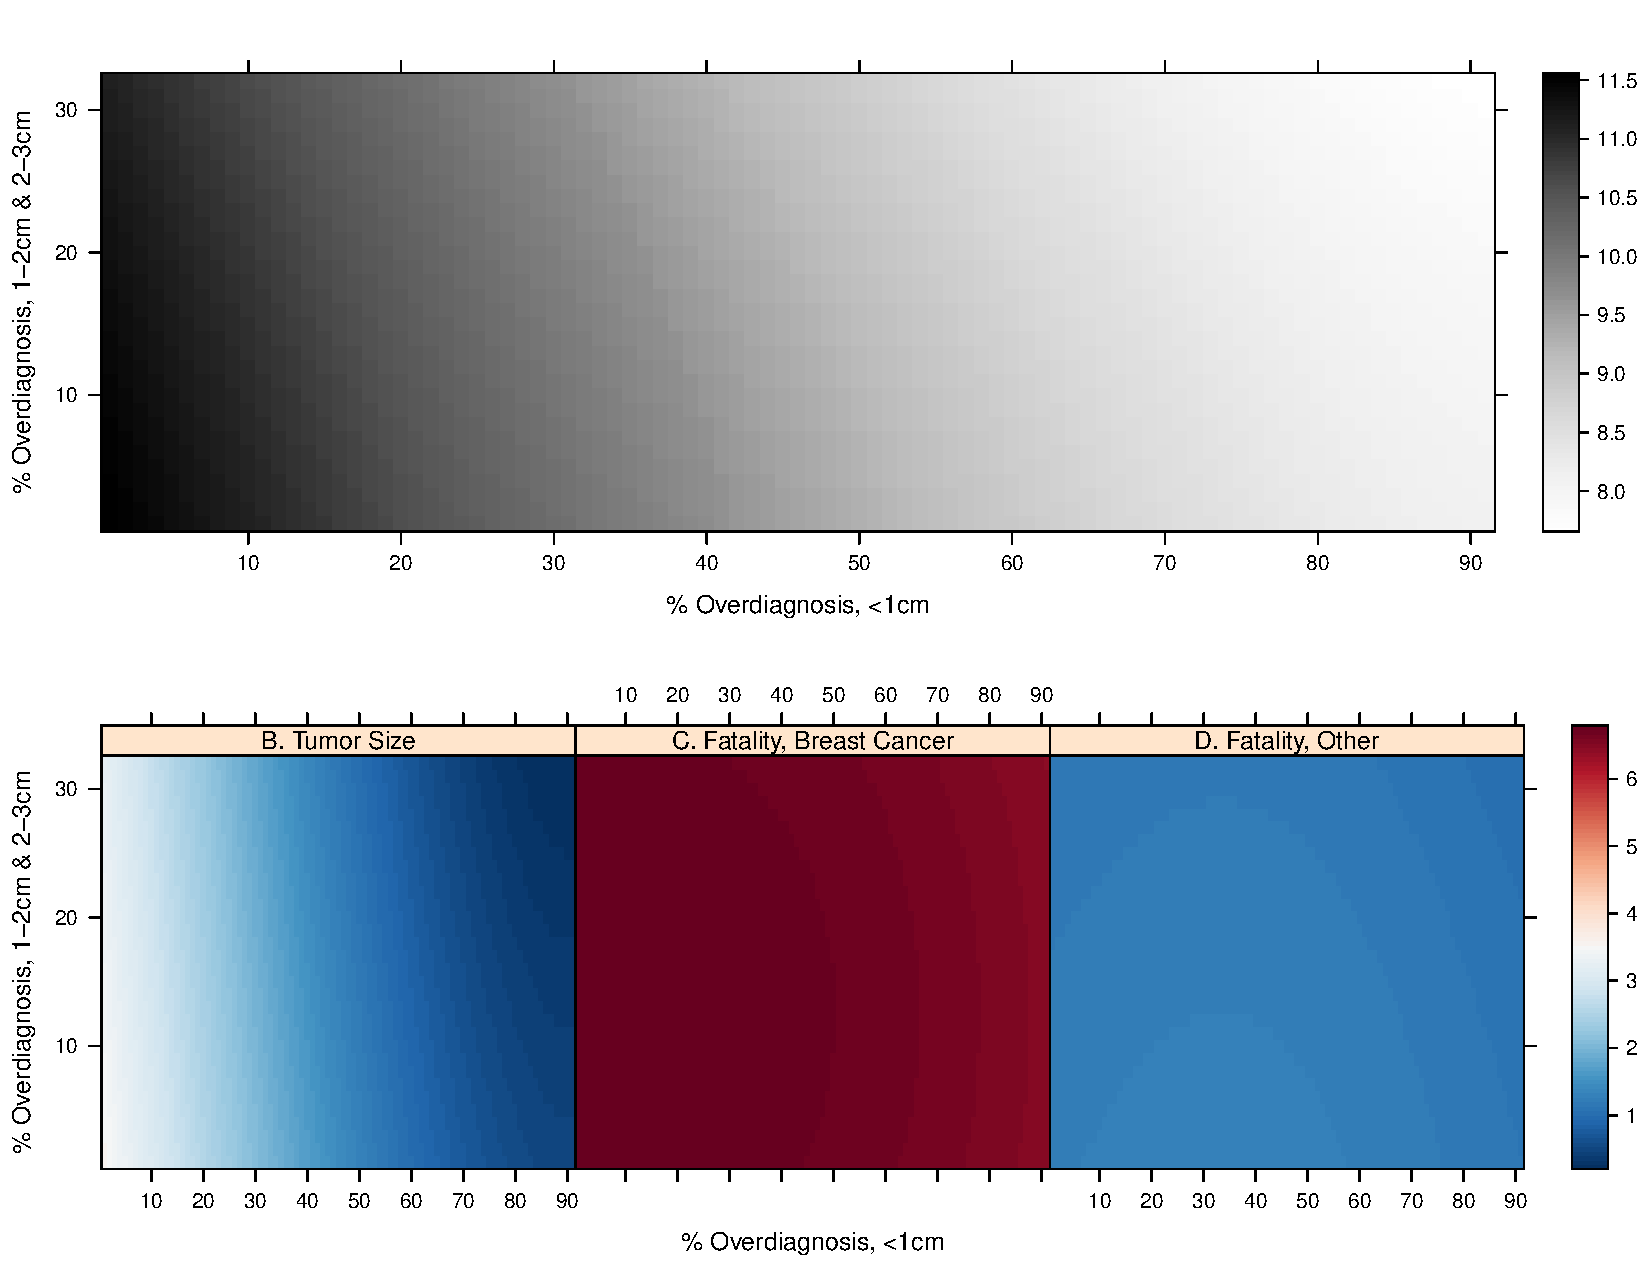
\includegraphics[scale=0.46]{appendix_figure2}
\spacingset{1}\caption{Gain in life expectancy (top panel) and
  contributions of the temporal shift to smaller sized tumors (bottom
  left), temporal reductions in case fatality rates from breast cancer
  (bottom center), and temporal reductions in case fatality rates from
  competing causes of death (bottom right) varying the overdiagnosis
  level for $<$1cm tumors (0\% to 90\%) and 1-3cm tumors (0\% to
  31\%).  The color scale for the top (bottom) panel indicates the
number of years of the gain in life expectancy (contribution to the gain).}
\label{fig:figure2}
\end{center}
\end{figure}

\newpage
\newpage
\section{Varying Time Intervals Between Diagnosis and Death}
\spacingset{1}
\begin{center}
  \begin{table}[h]
\begin{tabular}{@{}l rrrr@{}}
  Time & Gain in Life & &
                                \multicolumn{2}{c}{\underline{Reductions
                                in Case Fatality Rates from}}\\
  Interval & Expectancy & Tumor Size  & Breast Cancer   & Competing Causes  \\ 
  \midrule
  8  & 11.23 & 3.15 (28\%) & 7.07 (63\%) & 1.03 (9\%) \\ 
  9  & 10.93 & 3.09 (28\%) & 6.76 (62\%) & 1.09 (10\%) \\ 
  10  & 10.69 & 2.99 (28\%) & 6.57 (61\%) & 1.15 (11\%) \\ 
  11  & 10.38 & 2.78 (27\%) & 6.27 (60\%) & 1.35 (13\%) \\ 
  12  & 10.28 & 2.65 (26\%) & 6.05 (59\%) & 1.59 (15\%) \\ 
  \bottomrule
\end{tabular}
\caption{Gain in life expectancy and contribution of the temporal shift to smaller sized tumors, temporal reductions in case fatality rates from breast cancer, and temporal reductions in case fatality rates from
  competing causes of death, 1975-2000, varying time interval between breast
  cancer diagnosis and death.  Note: Yrs=years.}
\end{table}
\end{center}

\newpage\spacingset{1} \pdfbookmark[1]{References}{References}
\bibliography{cancer}
\end{document}



